\documentclass[11pt,a4paper]{article}

\usepackage[margin=2.5cm]{geometry}
\usepackage[utf8]{inputenc}
\usepackage[T1]{fontenc}
\usepackage{hyperref}
\usepackage{listings}
\usepackage{xcolor}
\usepackage{amsmath}
\usepackage{booktabs}
\usepackage{parskip}
\usepackage{enumitem}
\usepackage{graphicx}
\usepackage{caption}

\hypersetup{
    colorlinks=true,
    linkcolor=blue!50!black,
    urlcolor=blue!50!black,
    citecolor=blue!50!black,
    pdftitle={Antarctic Weather Platform: Technical Report},
    pdfauthor={M\'aria Nyolcas}
}

\definecolor{codebg}{rgb}{0.96,0.96,0.96}
\definecolor{codekeyword}{rgb}{0.0,0.0,0.6}
\definecolor{codestring}{rgb}{0.6,0.0,0.0}
\definecolor{codecomment}{rgb}{0.3,0.5,0.3}

\lstdefinestyle{pythonstyle}{
    language=Python,
    backgroundcolor=\color{codebg},
    basicstyle=\ttfamily\footnotesize,
    keywordstyle=\color{codekeyword}\bfseries,
    stringstyle=\color{codestring},
    commentstyle=\color{codecomment}\itshape,
    numbers=left,
    numberstyle=\tiny\color{gray},
    numbersep=8pt,
    frame=single,
    rulecolor=\color{gray!40},
    breaklines=true,
    showstringspaces=false,
    tabsize=4,
    captionpos=b,
}
\lstset{style=pythonstyle}

\title{\textbf{Antarctic Weather Platform}\\
\large Technical Report}
\author{M\'aria Nyolcas}
\date{}

\begin{document}

% --- Cover page ---
\begin{titlepage}
\centering
\vspace*{3cm}

{\Huge\bfseries Antarctic Weather Platform\par}
\vspace{0.5cm}
{\Large Technical Report\par}

\vspace{2cm}

{\large A backend and frontend system for retrieving, caching, aggregating,\\
and visualizing historical Antarctic meteorological observations\\
from AEMET OpenData\par}

\vfill

{\large\bfseries M\'aria Nyolcas\par}
\vspace{0.3cm}
{\large Prepared for GS Inima Environment\par}

\vspace{1.5cm}

{\large Development period: 21--28 August 2026\par}

\vspace{2cm}

\end{titlepage}

% --- Abstract, on its own page ---
\newpage
\begin{abstract}
\noindent This report documents the engineering reasoning behind a backend
and frontend system for retrieving, caching, aggregating, and visualizing
historical Antarctic meteorological observations from AEMET OpenData, built
for GS Inima Environment's evaluation of a hypothetical wind-farm project in
Antarctica. It complements the repository's \texttt{README.md}, which covers
setup, usage, and a summary of design decisions, by explaining \emph{why}
each non-trivial decision was made, including the alternatives considered
and their trade-offs. Source excerpts are referenced by file path and line
range against the repository at the time of writing, so every claim here can
be checked directly against running code, not reconstructed from memory.

\medskip
\noindent\textbf{A note on scope and timing}
\\[0.3em]
\noindent This report was written incrementally, alongside development,
rather than after the fact: a deliberate choice that carried a real
trade-off while the system was still in motion. Earlier revisions marked
sections depending on unfinished code with a visible \texttt{TODO} rather
than filling them with speculative content, and, for a period, stated
plainly that no CI pipeline existed rather than describing one that had
not yet been built. By this revision, every subsystem described below
(the AEMET integration, timezone and DST handling, aggregation, SQLite
caching, the frontend, the test suite, and continuous integration itself,
Section~\ref{sec:ci}) is complete, and every section is written against
the actual, running configuration, not intent.
\end{abstract}

\newpage
\tableofcontents
\listoffigures
\newpage

\section{Executive Summary}

The system exposes a single primary endpoint, \texttt{GET /observations},
that retrieves historical weather observations for one of two Spanish
Antarctic research stations (Gabriel de Castilla, Juan Carlos I) over a
caller-specified date range, optionally aggregated to hourly, daily, or
monthly resolution, and returns temperature, pressure, and wind speed in a
consistent, timezone-normalized shape.

Three engineering concerns dominated the design, in the order the challenge
itself weights them:

\begin{enumerate}[nosep]
    \item \textbf{Correctness under real-world data conditions.} AEMET's
    actual API behavior, including a two-step response indirection, a
    \texttt{"NaN"} string sentinel for missing measurements, an
    undocumented data-quality flag, and station-dependent optional fields,
    was verified against the live API before any client code was written,
    rather than assumed from the endpoint's description alone
    (Section~\ref{sec:aemet-integration}).
    \item \textbf{Temporal correctness.} The system distinguishes an
    instant, a local wall-clock representation, a named timezone's DST
    rules, and a fixed UTC offset as four genuinely different concepts,
    and handles the two DST edge cases (nonexistent and ambiguous local
    times) explicitly rather than relying on Python's implicit defaults
    (Section~\ref{sec:timezone-dst}).
    \item \textbf{A caching strategy whose behavior is fully explainable.}
    Rather than a general interval-coverage algorithm, the cache uses a
    deliberately scoped single-range containment check, reasoned through
    as a trade-off between completeness and explainability
    (Section~\ref{sec:caching}).
\end{enumerate}

\section{Requirements Analysis}
\label{sec:requirements}

\subsection{Source of truth}

The authoritative requirements are the official challenge specification
(PDF, three parts) together with direct clarification from the hiring
contact. Where the two could be read differently, the original PDF is
treated as authoritative, since it is the actual assessment document rather
than a paraphrase of it.

\subsection{Core functional requirements, as specified}

\begin{itemize}[nosep]
    \item A Python web API (FastAPI or Flask) exposing the AEMET Antarctic
    endpoint's data.
    \item Caller-specified start and end datetime
    (\texttt{AAAA-MM-DDTHH:MM:SS}).
    \item An optional location/timezone parameter, expressible either as
    an IANA timezone name (e.g. \texttt{Europe/Berlin}) or as a fixed UTC
    offset (e.g. \texttt{+02:00}).
    \item A choice of exactly two supported stations: ``Gabriel de
    Castilla'' and ``Juan Carlos I''.
    \item A time-aggregation selector: None, Hourly, Daily, or Monthly,
    with daily/monthly aggregation required to respect the meteo
    station's timezone rather than grouping raw UTC timestamps.
    \item Zero to three requested measurement types (temperature,
    pressure, wind speed); zero selected means all three are returned.
    \item Output datetimes in \texttt{Europe/Madrid} (CET/CEST), always
    carrying an explicit UTC offset.
    \item Explicit confirmation of DST behavior.
    \item SQLite persistence to avoid redundant upstream requests, with
    attention to database best practice, motivated explicitly by an
    anticipated high-volume, latency-sensitive consumer (intraday
    traders).
    \item Structured logging for troubleshooting.
    \item Automated tests, not required to be exhaustive.
    \item A frontend allowing the data to be queried and viewed in a
    table, optionally a chart, with explicit permission to use any
    reasonable technology stack.

\end{itemize}

\subsection{Ambiguities identified before implementation}

The specification is precise about behavior but silent on several
implementation-level questions that materially affect correctness. Each was
resolved deliberately, documented as an assumption, and isolated behind a
narrow interface so it can be revisited without a wider rewrite.

\begin{description}
    \item[Aggregation statistic.] The specification requires aggregation
    but does not name a statistic. Arithmetic mean was chosen for all
    three measurements (Section~\ref{sec:aggregation}); a second question
    --- whether wind speed specifically should also report a maximum,
    given the wind-farm context --- was raised with the assigning team
    rather than decided unilaterally, since it changes the response
    contract.
    \item[Default input timezone.] The specification marks the timezone
    parameter optional without stating a default. \texttt{Europe/Madrid}
    was chosen over UTC specifically because it keeps an unspecified date
    range aligned with the same calendar day in the (unconditionally
    Madrid) output, rather than spilling across a day boundary --- a
    concrete failure mode that was worked through with a numeric example
    before the decision was made.
    \item[Data-quality flag.] AEMET's live response includes a
    \texttt{qdato} field (data quality, 0 = good, 1 = bad) that is not
    part of the specification's field table. Its existence was discovered
    only by making a live API call, not by reading documentation. Whether
    a flagged-bad reading should be silently excluded from aggregation
    or exposed unfiltered was likewise raised with the assigning team.
    \item[Cache staleness.] The specification states AEMET's Antarctic
    dataset updates only a few times a year, but does not say whether a
    previously cached range should ever be considered stale and
    re-fetched. The current implementation caches a fetched range
    indefinitely; whether a revalidation window is expected was raised
    with the assigning team rather than assumed.
\end{description}

\subsection{Assumptions requiring verification}

Two further points were resolved by direct experimentation against the live
AEMET API rather than left as assumptions, and are recorded here because
they materially shaped the client and domain model:

\begin{itemize}[nosep]
    \item Whether the AEMET Antarctic endpoint returns data directly or
    via an indirection (a documented risk called out by the assigning
    team) --- confirmed to be a two-step indirection
    (Section~\ref{sec:aemet-integration}).
    \item The exact station identifiers for the two required stations,
    and whether the field schema is uniform across them --- confirmed via
    AEMET's own OpenAPI specification and a live request per station; the
    two stations were found \emph{not} to return an identical field set
    (Section~\ref{sec:aemet-integration}).
\end{itemize}

\section{Architecture}
\label{sec:architecture}

\subsection{Layering, and the requirement it serves}

The backend is organized into five layers, each with one responsibility:

\begin{center}
\begin{tabular}{@{}ll@{}}
\toprule
\textbf{Layer} & \textbf{Responsibility} \\
\midrule
API / Routes & Request validation, HTTP concerns, response shaping \\
Application / Service & Orchestration: cache check $\rightarrow$ AEMET fetch $\rightarrow$ aggregate \\
Domain & Pure functions: timezone conversion, aggregation, quality filtering \\
Repositories / Integrations & AEMET client, SQLite repository \\
External systems & SQLite, AEMET OpenData \\
\bottomrule
\end{tabular}
\end{center}

This is not layering for its own sake. The concrete requirement it serves is
testability under the specific correctness risks this system has: the
domain layer (\texttt{app/domain/time.py}, \texttt{app/domain/aggregation.py})
has \emph{no} dependency on FastAPI, SQLAlchemy, or httpx, so the timezone
and DST logic --- the single riskiest part of this system, per
Section~\ref{sec:timezone-dst} --- can be unit tested by constructing plain
Python \texttt{datetime} values and asserting on plain return values,
without a database, an HTTP mock, or a running application. The same is
true of the aggregation module. A change to how AEMET responses are parsed,
or how the API formats a response, cannot silently change how a DST
transition is handled, because the code paths do not intersect.

\subsection{Orchestration and dependency injection}

The application/service layer is a single class,
\texttt{WeatherService} (\texttt{backend/app/services/weather\_service.py}),
whose entire responsibility is sequencing: check whether the requested
range is cached, call AEMET only on a miss, persist the result, then
aggregate and return. It depends on its collaborators through its
constructor rather than constructing them itself:

\begin{lstlisting}[caption={\texttt{WeatherService} depends on an AEMET source through a \texttt{Protocol}, not the concrete client class. \texttt{backend/app/services/weather\_service.py}, lines 12--29.}]
class AemetObservationSource(Protocol):
    """The subset of AemetClient this service needs, lets tests substitute a fake with no real HTTP client behind it."""

    async def get_observations(
        self, station: Station, start: datetime, end: datetime
    ) -> list[StationObservation]: ...


class WeatherService:
    """Orchestrates cache lookup, AEMET retrieval, and aggregation."""

    # Exceptions from either collaborator propagate unchanged; mapping
    # them to HTTP responses is the API layer's job, not this one's.
    def __init__(
        self, aemet_client: AemetObservationSource, repository: ObservationRepository
    ) -> None:
        self._aemet_client = aemet_client
        self._repository = repository
\end{lstlisting}

This is a direct application of dependency inversion, chosen deliberately
over the alternative of having \texttt{WeatherService} import and
instantiate \texttt{AemetClient} directly. The concrete alternative that
was rejected --- constructing the real client inside the service and
mocking \texttt{httpx} at the transport level in every service test ---
would work, but it means every service-layer test also exercises (and can
be broken by) HTTP mocking concerns that have nothing to do with the
orchestration logic actually being tested. Depending on a \texttt{Protocol}
means the test suite's fake client
(\texttt{FakeAemetClient}, \texttt{tests/unit/test\_weather\_service.py},
lines 16--27) is a small class with no knowledge of HTTP at all, and ---
because \texttt{Protocol} is structurally typed --- \texttt{mypy} verifies
that both the fake and the real \texttt{AemetClient} satisfy the same
interface, so this is a property enforced by the type checker, not merely
true by convention.

\subsection{Three model shapes, not one}

A single AEMET observation is represented by three distinct types as it
moves through the system, and this distinction is deliberate rather than
incidental:

\begin{enumerate}[nosep]
    \item \textbf{Transport DTO} (\texttt{AemetObservationDTO},
    \texttt{app/integrations/aemet/schemas.py}) --- mirrors AEMET's actual
    wire format, including its quirks (Section~\ref{sec:aemet-integration}).
    \item \textbf{Domain model} (\texttt{StationObservation}, same file) ---
    a frozen, verified, in-domain reading with no knowledge of AEMET's
    field names or serialization conventions.
    \item \textbf{API response model} (\texttt{ObservationResponse},
    \texttt{app/api/schemas.py}) --- the wire contract this application
    exposes, independent of both AEMET's format and the internal domain
    representation.
\end{enumerate}

Collapsing these into one type would couple three independently-changing
concerns: AEMET could alter its response format, the internal
representation could be refactored for a new aggregation strategy, and the
public API contract could evolve for frontend needs --- none of which
should require touching the other two.

\section{AEMET Integration}
\label{sec:aemet-integration}

\subsection{What had to be verified before writing the client}

The challenge specification flagged the AEMET Antarctic endpoint as
carrying real integration risk, without saying exactly what that risk was.
Three concrete unknowns were resolved against the live API, using a
personal AEMET OpenData API key, before any client code was written, on the
principle that a typed client built against an assumed shape would need to
be rewritten anyway the moment reality disagreed:

\begin{enumerate}[nosep]
    \item \textbf{Response indirection.} AEMET's Antarctic endpoint
    (\texttt{GET /api/antartida/datos/fechaini/\{...\}/fechafin/\{...\}
    /estacion/\{...\}}) does not return observation data directly. It
    returns a small JSON envelope containing two pre-signed URLs,
    \texttt{datos} (the actual records) and \texttt{metadatos} (field
    documentation), which must be fetched with a second HTTP call. This
    two-step shape is common across AEMET OpenData endpoints generally but
    is not obvious from the Antarctic endpoint's own documentation page,
    and was confirmed by making a real request and inspecting the response
    body directly.
    \item \textbf{The \texttt{datos} URL does not take the API key.} The
    pre-signed link AEMET issues in the envelope is itself the
    authentication mechanism for the second request; attaching the
    \texttt{api\_key} header (correct for the first call) to the second
    call was tried and made no difference, confirming the header is simply
    ignored on that endpoint rather than rejected, which is why
    \texttt{\_request\_records} (\texttt{client.py}, lines 113--128) passes
    \texttt{headers=None} explicitly rather than omitting the parameter by
    accident.
    \item \textbf{Station identifiers and field uniformity.} The two
    required station names, ``Gabriel de Castilla'' and ``Juan Carlos I'',
    are not self-evidently mapped to AEMET's internal station codes.
    Cross-referencing AEMET's published OpenAPI specification against a
    live request per station confirmed \texttt{89070} and \texttt{89064}
    respectively, and, more importantly, revealed the two stations do
    \emph{not} return an identical field set: Juan Carlos I's live response
    included \texttt{radKjM2}, \texttt{rec}, \texttt{tsb}, and
    \texttt{altNieve} fields entirely absent from Gabriel de Castilla's.
    Had the transport DTO been written to expect a fixed field set, this
    would have surfaced as a runtime validation failure against exactly one
    of the two required stations, in production, rather than being caught
    at the boundary. The mapping layer instead treats every field outside
    the five actually used (station identifier, timestamp, temperature,
    pressure, wind speed, plus the quality flag below) as optional and
    ignored.
\end{enumerate}

\subsection{Undocumented behavior discovered only by live testing}

Two further AEMET behaviors were never documented anywhere in the
specification or the OpenAPI file, and would have produced either silently
wrong data or a confusing failure if the client had been written against
documentation alone.

\textbf{The quality flag.} Every observation record carries a
\texttt{qdato} field (0 = good, 1 = bad), not part of the challenge's
stated field table. Its existence was discovered only by inspecting a live
response body. Whether a flagged-bad reading should be silently dropped or
surfaced as-is materially changes the API's output, so this was raised with
the assigning team rather than decided unilaterally (Section~\ref{sec:requirements}):
the resolution is that a \texttt{qdato = 1} reading is retained verbatim in
the SQLite cache (the cache is a faithful copy of what AEMET actually sent)
but reported as \texttt{null} for that measurement in every API response,
aggregated or not, since a flagged-bad value should never be presented to a
caller as trustworthy.

\textbf{The \texttt{"NaN"} sentinel.} AEMET represents an inapplicable or
missing numeric field as the literal JSON string \texttt{"NaN"}, not a JSON
\texttt{null} and not an omitted key. A transport model expecting a numeric
type or \texttt{null} would raise a validation error on any record
containing this sentinel, which is common enough (not every station reports
every field on every reading) that it would have broken ordinary queries,
not just edge cases. This is intercepted explicitly in the DTO-to-domain
mapping, before any numeric coercion is attempted, converting the literal
string to \texttt{None} rather than letting it reach a
\texttt{float()} call or a Pydantic numeric validator.

\subsection{Two distinct meanings of \texttt{estado: 404}, and why conflating them would be a silent bug}

AEMET signals ``no data available for this range'' in two different ways,
both found empirically rather than documented:

\begin{enumerate}[nosep]
    \item A genuine HTTP \texttt{404} status code, handled by the caller
    before the envelope is even parsed (\texttt{\_request\_envelope},
    lines 96--111).
    \item An HTTP \texttt{200} response whose JSON body carries
    \texttt{estado: 404} with no \texttt{datos}/\texttt{metadatos} fields
    at all.
\end{enumerate}

The second form is also, confusingly, the exact same wrapper AEMET uses
when a request is rejected for spanning more than its undocumented
$\sim$31-day maximum range (\texttt{"El rango de fechas no puede ser
superior a 1 mes"}). This was discovered by querying a full year of data
and receiving far fewer observations than expected, silently, with no error
raised, because the naive interpretation of \texttt{estado: 404} as ``empty
result'' swallowed the actual problem (a rejected, oversized request) and
reported it as if AEMET simply had no data for most of the year. Treating
these as the same case would be a genuine correctness bug, not a coarse
approximation: it would make a query silently return a small, wrong subset
of a valid range while reporting success. \texttt{\_parse\_envelope}
(\texttt{client.py}, lines 206--232) distinguishes the two by inspecting
the \texttt{descripcion} text for the range-length phrase before falling
back to treating the response as a legitimate empty result, and raises
\texttt{AemetRangeTooLongError} rather than returning \texttt{[]} when it
matches:

\begin{lstlisting}[caption={Disambiguating two meanings of the same wrapper. \texttt{backend/app/integrations/aemet/client.py}, lines 221--225.}]
if isinstance(body, dict) and body.get("estado") == 404:
    descripcion = body.get("descripcion", "")
    if isinstance(descripcion, str) and "rango de fechas" in descripcion.lower():
        raise AemetRangeTooLongError(descripcion)
    return None
\end{lstlisting}

Because \texttt{WeatherService} proactively splits every requested range
into $\le$31-day chunks before calling the client at all
(Section~\ref{sec:caching}), \texttt{AemetRangeTooLongError} should never
actually surface during normal operation; it exists so that if that
invariant is ever violated by a future change, the client fails loudly with
a distinct, named exception rather than silently misreporting a rejected
request as an empty one.

\subsection{Retry and rate-limiting strategy}
\label{sec:retry-strategy}

AEMET does not publish a rate limit for this endpoint. Per explicit
guidance from the assigning team, the chosen response to an undocumented
limit is to behave conservatively rather than to guess a threshold and tune
against it empirically. The client applies two independent mechanisms:

\textbf{Proactive throttling.} Every outbound request, regardless of
outcome, passes through a single choke point
(\texttt{\_throttled\_get}, lines 177--185) enforcing a minimum 500ms
spacing from the previous request. This is guarded by an
\texttt{asyncio.Lock}, not merely a plain variable check, because an
unsynchronized ``has enough time passed?'' check followed by a sleep is a
classic check-then-act race: two concurrent callers could both observe
that enough time has elapsed and fire simultaneously, defeating the
throttle exactly when it matters most (concurrent load).

\textbf{Reactive backoff on a real 429.} A single retry after a fixed delay
is sufficient for the generic 5xx/timeout case (Section~\ref{sec:aemet-general-retry}
below), but a 429 specifically needed more. \texttt{WeatherService} splits
any range over $\sim$31 days into sequential chunked requests
(Section~\ref{sec:caching}), so a single wide query can issue dozens of
requests to AEMET in a row; this was confirmed live to be able to trip
AEMET's undocumented limit more than once within a single logical query,
not just once at the start. A single retry, tried first, was empirically
insufficient: verified directly by running the exact 26-month query that
had been failing and observing that a real 429 could still occur again
after the first retry succeeded. The fix retries up to three times, with
the cooldown doubling on each consecutive attempt (5s, 10s, 20s by
default):

\begin{lstlisting}[caption={Multi-retry 429 handling with a doubling cooldown. \texttt{backend/app/integrations/aemet/client.py}, lines 146--167.}]
if response.status_code == 429:
    for attempt in range(1, _MAX_RATE_LIMIT_RETRIES + 1):
        cooldown = self._rate_limit_cooldown_seconds * (2 ** (attempt - 1))
        self._apply_rate_limit_cooldown(cooldown)
        logger.warning(
            "AEMET returned 429, retry %d/%d after %.1fs cooldown: %s",
            attempt, _MAX_RATE_LIMIT_RETRIES, cooldown, url,
        )
        await asyncio.sleep(cooldown)
        response = await self._throttled_get(url, headers=headers)
        if response.status_code != 429:
            break
\end{lstlisting}

This was verified end-to-end against the live API, not only against mocked
429 responses in the unit test suite: the same 26-month query that had
previously failed outright was re-run against production AEMET after the
fix, encountered one real 429 partway through its sequence of chunked
requests, retried successfully on the first attempt, and completed with
109{,}832 observations returned, confirmed against the backend's own log
output rather than assumed from a lack of visible error. A 429 that
persists through all three retries still raises
\texttt{AemetUnavailableError} rather than retrying indefinitely, since an
AEMET-side block that outlasts a 35-second total backoff window is a
genuine outage, not a transient collision.

\subsection{Generic retry for transport and server failures}
\label{sec:aemet-general-retry}

Connection failures, timeouts, and 5xx responses are retried exactly once,
after a short fixed delay, deliberately not the same doubling-backoff
strategy used for 429s. The reasoning is proportionality to what this
application actually is: a single-user local service, not a distributed
system fielding concurrent load from many clients, so a transient network
blip is the failure mode being guarded against, not a shared upstream
buckling under aggregate pressure that would call for exponential backoff.
A second attempt either succeeds quickly or the caller learns AEMET is
genuinely unavailable and receives \texttt{AemetUnavailableError} rather
than waiting through several escalating delays for a condition unlikely to
self-resolve on this timescale. 401/403 responses (a rejected or missing
API key) are never retried and raise \texttt{AemetAuthenticationError}
instead, kept as a distinct exception from \texttt{AemetUnavailableError}:
a bad key is a configuration problem that retrying cannot fix, and
conflating the two would give any future retry-on-failure logic upstream
the wrong answer to ``is this worth trying again?''

\section{Timezone and DST Handling}
\label{sec:timezone-dst}

\subsection{Four concepts, not one}

The specification requires the system to accept an optional timezone (as
either an IANA name or a fixed UTC offset), always output
\texttt{Europe/Madrid} regardless of the input, and explicitly confirm DST
behavior. Meeting this correctly requires keeping four genuinely different
concepts distinct throughout the pipeline, rather than treating
``timezone'' as one idea with several representations:

\begin{enumerate}[nosep]
    \item A \textbf{naive wall-clock value}: what a caller types
    (\texttt{2026-03-29T02:30:00}), meaningless as an instant in time until
    paired with a timezone.
    \item A \textbf{named timezone} (\texttt{zoneinfo.ZoneInfo}): an IANA
    DST rule set that produces a different UTC offset on different
    calendar dates, not a fixed number.
    \item A \textbf{fixed UTC offset} (e.g.\ \texttt{+02:00}): exactly that
    many hours from UTC on every date supplied, carrying no DST logic at
    all. This is not a simplified way of writing ``Europe/Madrid in
    summer''; it is a different kind of object entirely, and a caller
    using this form is opting out of DST reasoning explicitly, a
    consequence stated directly in the code comment above
    \texttt{\_UTC\_OFFSET\_PATTERN} (\texttt{time.py}, lines 14--19).
    \item The \textbf{UTC instant} that a (wall-clock, timezone) pair
    resolves to, and the \textbf{Europe/Madrid output representation} of
    that same instant, which is unconditional: every response datetime is
    Europe/Madrid regardless of what timezone the request specified.
\end{enumerate}

Collapsing any two of these would reintroduce exactly the class of bug this
system is trying to rule out: for instance, treating a fixed offset as
interchangeable with an IANA name would make a caller's \texttt{+01:00}
input silently behave as if it carried Madrid's DST rules on a date where
Madrid is actually at \texttt{+02:00} (CEST), producing a response an hour
off from what was actually requested with no error raised anywhere.

\subsection{Resolving a timezone input}

\texttt{resolve\_timezone} (\texttt{time.py}, lines 23--33) tries the fixed
UTC offset pattern first, falling back to \texttt{ZoneInfo} construction,
and raises \texttt{InvalidTimezoneError} (mapped to HTTP 400) for anything
that matches neither form, rather than letting an unrecognized string
propagate as an unhandled \texttt{ZoneInfoNotFoundError} deep inside the
conversion pipeline:

\begin{lstlisting}[caption={Two accepted timezone forms, tried in order. \texttt{backend/app/domain/time.py}, lines 23--33.}]
def resolve_timezone(name: str) -> tzinfo:
    offset_match = _UTC_OFFSET_PATTERN.match(name)
    if offset_match:
        sign, hours, minutes = offset_match.groups()
        delta = timedelta(hours=int(hours), minutes=int(minutes))
        return timezone(-delta if sign == "-" else delta)

    try:
        return ZoneInfo(name)
    except ZoneInfoNotFoundError as exc:
        raise InvalidTimezoneError(name) from exc
\end{lstlisting}

\subsection{The two DST hazards, handled explicitly rather than left to Python's defaults}

Python's \texttt{datetime} module does not, by default, protect a caller
from either DST edge case; both are handled explicitly in
\texttt{to\_utc\_instant} (\texttt{time.py}, lines 36--55) rather than
relying on whatever \texttt{zoneinfo} happens to pick.

\textbf{Nonexistent local times.} During a spring-forward transition (in
2026, confirmed empirically against Python's own \texttt{zoneinfo} data
rather than assumed, Europe/Madrid's clocks jump from 02:00 to 03:00 on 29
March), a wall-clock time inside the skipped hour, e.g.\
\texttt{2026-03-29T02:30:00}, never actually occurs. Python does not
reject this at construction time; it silently assigns it some UTC offset
and lets the program proceed as if the time were valid. The function
detects this by round-tripping the candidate value through UTC and back:
if converting to UTC and back to the same named timezone does not reproduce
the original wall-clock value bit-for-bit, the value was never real, and
\texttt{NonexistentLocalTimeError} is raised (mapped to HTTP 400) rather
than silently returning whichever instant \texttt{zoneinfo}'s default
\texttt{fold=0} behavior happened to produce:

\begin{lstlisting}[caption={Detecting a spring-forward gap by round-tripping. \texttt{backend/app/domain/time.py}, lines 45--55.}]
aware = local_dt.replace(tzinfo=tz, fold=0)

round_tripped = aware.astimezone(ZoneInfo("UTC")).astimezone(tz)
if round_tripped.replace(tzinfo=None) != local_dt:
    raise NonexistentLocalTimeError(local_dt.isoformat(), str(tz))

return aware.astimezone(ZoneInfo("UTC"))
\end{lstlisting}

\textbf{Ambiguous local times.} During the fall-back transition (Madrid's
clocks move from 03:00 back to 02:00 on 25 October 2026), the wall-clock
hour between 02:00 and 03:00 occurs twice: once at UTC+2 (CEST, before the
transition) and once at UTC+1 (CET, after it). Python's \texttt{fold}
attribute distinguishes the two occurrences, but leaving the default
(\texttt{fold=0}) unaddressed would mean the choice is made by a Python
implementation detail rather than a documented decision. This system
resolves every ambiguous time to its \emph{first} occurrence
(pre-transition, \texttt{fold=0}) explicitly, as a stated convention, not
an implicit default the caller has to discover by reading CPython source.

Both transition dates for 2026 were verified against Python's installed
\texttt{zoneinfo} (IANA tz database) directly, not assumed from a general
rule about ``last Sunday of March/October'', and both hazards are covered
by tests anchored to those exact calendar dates
(\texttt{backend/tests/unit/test\_domain\_time.py}), so a future tz
database update that shifted a transition date would be caught by a
failing test rather than silently changing behavior.

\subsection{Output representation}

\texttt{to\_output\_representation} (\texttt{time.py}, lines 58--66)
converts any aware instant to Europe/Madrid, unconditionally, and rejects a
naive input outright rather than guessing which timezone it might be in.
This is the only function in the pipeline responsible for producing the
representation callers actually see, so every response datetime, and every
aggregation bucket boundary, is computed by calling through this one
function rather than by ad hoc \texttt{.astimezone()} calls scattered
across the codebase.

\section{Aggregation Strategy}
\label{sec:aggregation}

\subsection{Bucket boundaries are drawn in Madrid local time, not UTC}

The specification requires that daily and monthly aggregation respect the
station's (i.e.\ Madrid's, per the fixed output timezone) local calendar,
not raw UTC grouping. This matters concretely, not just as a stated rule:
because Madrid's UTC offset is never zero (+01:00 CET or +02:00 CEST), a
boundary drawn against raw UTC timestamps would routinely split
observations that belong to the same Madrid calendar day into two
different buckets, or merge observations from two different Madrid days
into one, depending on the time of year and time of day. \texttt{aggregate}
(\texttt{aggregation.py}, lines 78--131) converts every observation to its
Madrid representation \emph{before} computing a bucket key
(\texttt{\_bucket\_key}, lines 46--53), so the grouping key is always a
local calendar tuple (year, month, day, hour for hourly; year, month, day
for daily; year, month for monthly), never a UTC timestamp:

\begin{lstlisting}[caption={Bucket keys are Madrid calendar tuples. \texttt{backend/app/domain/aggregation.py}, lines 100--104.}]
for obs in observations:
    local_dt = to_output_representation(obs.observed_at)
    key = _bucket_key(local_dt, level)
    buckets[key].append(obs)
    bucket_starts.setdefault(key, _bucket_start(key, local_dt))
\end{lstlisting}

This is tested directly rather than trusted by inspection: two
observations exactly one hour apart in UTC, straddling a Madrid local
midnight, are asserted to land in different daily buckets, and the same
scenario is repeated across the March 2026 DST transition date to confirm
the bucket key tracks the local calendar date through the offset change,
not a fixed-width UTC split (\texttt{test\_domain\_aggregation.py}).

\subsection{Why the mean, and why wind speed additionally reports a maximum}

The specification requires aggregation but names no specific statistic.
Arithmetic mean,
\[
\bar{x} = \frac{1}{n}\sum_{i=1}^{n} x_i,
\]
was chosen for all three measurements as the standard estimator of a
continuous physical quantity's typical value over an interval, appropriate
given AEMET's roughly regular $\sim$10-minute sampling interval. It is,
however, an explicitly incomplete summary on its own: averaging discards
information about variability within the bucket, most consequentially for
wind speed, where a bucket containing one strong gust amid mostly calm air
can share an identical mean with a bucket of steady, moderate wind.

This is not a purely statistical concern in this context. It was raised
with, and confirmed by, the assigning team: turbine power generation has
minimum (cut-in), maximum (cut-out), and optimal (rated) operating
wind-speed thresholds, so a mean alone can conceal a period whose actual
wind conditions were outside a turbine's safe or productive operating
range, which is directly load-bearing for a wind-farm feasibility
assessment in a way it is not for, say, an average temperature. The
resolution changes the response contract itself, not merely an internal
calculation: \texttt{AggregatedObservation} (lines 19--38) carries both
\texttt{wind\_speed\_ms} (the bucket mean) and \texttt{wind\_speed\_max\_ms}
(the bucket maximum) as separate fields, while temperature and pressure
report only their mean, since the same operational-threshold reasoning
does not apply to them in this context.

\subsection{Quality filtering happens once, at aggregation time}

AEMET's \texttt{qdato} flag is applied at exactly one point in the pipeline
(\texttt{aggregate}, not the repository layer): every mean and maximum is
computed only over readings where \texttt{is\_good\_quality} is true and
the value itself is not \texttt{None}. A bucket where every contributing
reading is missing or flagged bad reports \texttt{null} for that
measurement, deliberately never \texttt{0.0}: zero is a real, physically
meaningful value a sensor could legitimately report, so using it to mean
``no valid data'' would make a genuine zero-reading bucket
indistinguishable from an empty one, silently corrupting downstream
analysis (a chart, a mean-of-means) with no signal that anything was
wrong. Concentrating this filtering in one function, rather than applying
it once when data is cached and again when it is read back, means the
policy can be revisited (e.g.\ if the assigning team's stance on
flagged-bad data ever changed) without needing to re-fetch or migrate
anything already stored; \texttt{ObservationRepository.\_to\_domain}
(\texttt{repository.py}, lines 105--117) deliberately returns raw stored
values, unfiltered, so this single point of enforcement is not
duplicated or risked drifting out of sync.

\subsection{Sparse buckets, not padded ones}

\texttt{aggregate} only emits a bucket for a calendar period that contains
at least one raw observation; a gap in AEMET's own data (a missing hour, a
station outage) produces no row for that period at all, rather than a row
padded with \texttt{null}s to preserve a continuous time axis. This keeps
the function's contract simple, since it needs only the observations
themselves and never the originally requested range, and avoids
fabricating rows the source data never actually contained. The trade-off is
explicit: a chart or table consuming this response must not assume a
gap-free, evenly-spaced time axis, and the frontend's chart component
(Section~\ref{sec:frontend}) is written with that assumption in mind, most
visibly in not connecting a line across a \texttt{null} value.

\section{Persistence and Caching}
\label{sec:caching}

\subsection{Two tables, each tracking a different fact}

The schema (\texttt{backend/app/db/models.py}) has exactly two tables, and
each exists to answer a specific question the caching logic actually needs
answered, rather than being a generic denormalized store:

\textbf{\texttt{observations}} answers ``what did AEMET report for station
$X$ at instant $t$?'' Its identity is the pair \texttt{(station,
observed\_at)}: the same station measuring at the same instant is the same
observation by definition, which is enforced as an actual database
constraint,
\begin{lstlisting}[caption={The observation's real identity, enforced by the database, not just application convention. \texttt{backend/app/db/models.py}, lines 41--44.}]
__table_args__ = (
    UniqueConstraint("station", "observed_at", name="uq_observation_identity"),
    Index("ix_observation_station_time", "station", "observed_at"),
)
\end{lstlisting}
not merely an application-level convention that a caching bug could quietly
violate. The same composite column pair also serves as the query index,
since every real read is ``observations for station $X$ between times $A$
and $B$'', so the constraint and the index serve two purposes with one
structure.

\textbf{\texttt{fetched\_ranges}} answers a different question: ``was
AEMET ever asked about station $X$ for this range, regardless of what it
returned?'' This table is necessary specifically because AEMET publishes
this dataset with a real, variable lag behind the present. A recent date
range can legitimately have zero observations simply because AEMET has not
published that data yet, and without an explicit record that the range was
already queried, that state would be indistinguishable from ``this range
was never asked about'', which would cause every request for a recent
range to re-query AEMET on every call, defeating the cache's purpose for
exactly the queries most likely to be repeated (a user checking whether
new data has appeared).

\subsection{Cache-hit logic: single-range containment, chosen deliberately over a general interval algorithm}

For a requested range $R$ on a given station, \texttt{is\_range\_cached}
(\texttt{repository.py}, lines 18--33) checks whether $R$ is fully
contained within a \emph{single} previously fetched range, not whether $R$
is covered by the union of several stored ranges (a true interval-tree set
difference, $R \setminus \bigcup C_i$, across arbitrarily many stored
intervals). A request spanning two previously-fetched but non-adjacent
ranges is therefore treated as a full miss and re-fetched in its entirety,
even though part of that range is technically already present in
\texttt{observations}.

This is a deliberate, scoped trade-off, not an oversight. The actual usage
pattern this system serves, a user submitting and then refining one query
at a time, is well served by single-range containment: it is simple to
state, simple to verify by reading the query, and does not require
maintaining or periodically compacting a set of disjoint stored intervals.
A general interval-merging cache would be strictly more capable in the
abstract, but that capability is not free: it introduces a real algorithm
(interval merging or an interval tree) with its own edge cases (adjacent
but non-overlapping ranges, redundant sub-ranges, merge ordering) purely to
serve a usage pattern this application does not actually have. Reasoning
explicitly about proportionality here is the same judgment applied to the
layering decision in Section~\ref{sec:architecture} and the DDD scoping
decision in the README: correctness and explainability do not require the
more general mechanism at this scale, so it is not built.

\subsection{Chunking interacts with caching, not just with AEMET's range limit}

Because AEMET rejects any single request spanning more than $\sim$31 days
(Section~\ref{sec:aemet-integration}), \texttt{WeatherService.get\_observations}
splits every requested range into sequential $\le$31-day chunks
\emph{before} either the cache or AEMET is consulted, and checks the cache
independently for each chunk:

\begin{lstlisting}[caption={Cache coverage is checked per chunk, giving finer-grained reuse than the containment rule alone would suggest. \texttt{backend/app/services/weather\_service.py}, lines 82--94.}]
for chunk_start, chunk_end in _chunk_range(start, end):
    if self._repository.is_range_cached(station, chunk_start, chunk_end):
        logger.info("Cache hit for %s [%s, %s]", station.value, chunk_start, chunk_end)
        continue

    fetched = await self._aemet_client.get_observations(station, chunk_start, chunk_end)
    self._repository.store_fetch_result(station, chunk_start, chunk_end, fetched)
\end{lstlisting}

This has a consequence worth stating explicitly: although the containment
rule above is scoped to a single stored range, chunking makes the
\emph{effective} cache behavior finer-grained than that description alone
implies. A year-long request previously fetched one month at a time is
checked, and can hit, one month-sized chunk at a time; only the chunks not
already covered trigger a real AEMET call. A test asserts this directly,
storing one cached month inside a larger requested span and confirming
only the uncached remainder results in an AEMET call
(\texttt{test\_already\_cached\_chunk\_within\_a\_large\_range\_is\_not\_refetched},
\texttt{test\_weather\_service.py}).

\subsection{Two SQLite-specific correctness bugs, caught by tests rather than assumed away}

Two issues surfaced during development that would have been silent data
bugs, not crashes, had they gone unnoticed, and are recorded here because
both were caught by a failing test rather than anticipated in advance.

\textbf{Timezone loss on round-trip.} SQLite's \texttt{DATETIME} column
type has no concept of a timezone; SQLAlchemy, by default, returns a naive
\texttt{datetime} on read even when an aware value was written. A
round-trip test (write an aware UTC datetime, read it back, assert
\texttt{tzinfo} is still set) caught this directly: the value came back
missing its timezone entirely. Given the amount of this system built
specifically to keep timezone-aware and naive values from ever being
conflated (Section~\ref{sec:timezone-dst}), silently reintroducing a naive
value at the persistence boundary would have undermined that work in a way
that would not necessarily surface as a visible error, only as an
occasionally wrong answer. The fix, \texttt{UTCDateTime}
(\texttt{models.py}, lines 17--34), is a small SQLAlchemy
\texttt{TypeDecorator} that strips the timezone before writing (SQLite
cannot store it) and re-attaches UTC on every read, since every datetime
this application ever persists is UTC by construction; this makes the fix
a correctness guarantee actually enforced by a type, not a convention
relying on every call site remembering to reattach it manually.

\textbf{\texttt{Session.merge()} upserts on the wrong key.} An idempotency
test, re-fetching a range that overlapped a previously-stored one, was
expected to update the existing rows; instead it raised
\texttt{IntegrityError} against the \texttt{(station, observed\_at)}
unique constraint. The cause: SQLAlchemy's \texttt{Session.merge()} decides
insert-versus-update based on the ORM's primary key (\texttt{id}), and
every freshly constructed \texttt{ObservationRecord} coming back from a new
AEMET fetch has no \texttt{id} set yet, so \texttt{merge()} always treated
it as a new row regardless of whether the same \texttt{(station,
observed\_at)} pair already existed. The fix, in
\texttt{store\_fetch\_result} (\texttt{repository.py}, lines 69--102),
replaces \texttt{merge()} with an explicit
\texttt{INSERT ... ON CONFLICT (station, observed\_at) DO UPDATE}, which
targets the pair that is actually the observation's real business identity
rather than the ORM surrogate key, and both writes (the observation rows
and the \texttt{FetchedRange} marker) are wrapped in a single
\texttt{session\_scope} transaction so the two tables can never disagree
about what has been cached if one write succeeds and the other fails.

\subsection{Cache staleness: intentionally unbounded}

A fetched range is cached indefinitely; there is no TTL or revalidation
policy on the \texttt{observations} table. This was confirmed as correct
by the assigning team rather than assumed for convenience
(Section~\ref{sec:requirements}): AEMET's historical Antarctic dataset is
stable once published and does not change retroactively, so a
revalidation policy would add real complexity (a staleness clock, a
re-fetch trigger, cache-invalidation reasoning) to guard against a
condition that does not occur in this data source. This is a different
concern from the \texttt{get\_latest\_available\_date} endpoint's own
1-hour in-process TTL (Section~\ref{sec:latest-available}), which caches
the answer to a different, genuinely time-varying question, ``what is the
most recent date with data \emph{right now}'', not the historical
observations themselves.

\subsection{The \texttt{latest-available} endpoint}
\label{sec:latest-available}

A later addition to the system, \texttt{GET /observations/latest-available}
answers ``what is the most recent date AEMET is confirmed to have data
for?'', driving the frontend's date-picker cap so a query doomed to return
nothing is caught before submission rather than after. AEMET itself
exposes no such endpoint; it is a pure range-query API. The implementation
is cache-first: \texttt{MAX(observed\_at)} over the already-cached
\texttt{observations} table is both free (no network call) and already the
most authoritative record this application has of what data has actually
been confirmed to exist, since the cache is populated exclusively by
successful AEMET fetches. Only when nothing is cached yet for a station
(a cold start) does the service fall back to a live probe, stepping back
through 60-day windows for up to six attempts looking for the first window
that returns any data (\texttt{\_probe\_aemet\_for\_latest\_date},
\texttt{weather\_service.py}, lines 125--138), bounded so a station with no
AEMET coverage at all fails after a fixed number of attempts rather than
probing indefinitely. The endpoint's own answer is additionally cached
in-process for one hour per station, since the true value changes at most
roughly monthly in reality but this endpoint may be called on every
frontend page load.

\section{Testing Strategy}
\label{sec:testing}

\subsection{Backend: 142 tests, isolating the two riskiest subsystems}

The backend test suite (\texttt{backend/tests/}, pytest,
pytest-asyncio, \texttt{pytest\_httpx} for mocking AEMET HTTP calls) had
142 collected tests at the time of writing, organized to keep the
system's two highest-risk areas, timezone/DST conversion and aggregation,
testable in complete isolation from FastAPI, SQLAlchemy, and httpx:

\begin{center}
\begin{tabular}{@{}ll@{}}
\toprule
\textbf{File} & \textbf{Scope} \\
\midrule
\texttt{test\_domain\_time.py} & Timezone resolution, DST hazards, output representation \\
\texttt{test\_domain\_aggregation.py} & Bucketing, mean/max, quality filtering, DST-crossing buckets \\
\texttt{test\_aemet\_client.py} & Two-step flow, retries, 429 backoff, \texttt{estado: 404} disambiguation \\
\texttt{test\_aemet\_schemas.py} & DTO validation, \texttt{"NaN"} sentinel handling, domain mapping \\
\texttt{test\_db\_repository.py} & Cache hit/miss, upsert correctness, timezone round-trip \\
\texttt{test\_db\_models.py} & Schema constraints, \texttt{UTCDateTime} type behavior \\
\texttt{test\_weather\_service.py} & Chunking, cache-per-chunk, latest-available probing and TTL \\
\texttt{test\_config.py} & Startup validation of required/optional settings \\
\texttt{test\_exceptions.py} & Exception hierarchy shape \\
\texttt{test\_logging.py} & Logging configuration \\
\texttt{test\_main.py} & App factory, health check \\
\texttt{test\_observations\_route.py} & Full FastAPI app, end-to-end, AEMET mocked at the HTTP layer only \\
\bottomrule
\end{tabular}
\end{center}

The unit/integration boundary is deliberate: unit tests
(\texttt{tests/unit/}) exercise one module with everything else faked
(\texttt{FakeAemetClient} and \texttt{ScriptedAemetClient} in
\texttt{test\_weather\_service.py} implement the \texttt{AemetObservationSource}
protocol with no HTTP involved at all), while integration tests
(\texttt{tests/integration/test\_observations\_route.py}) exercise the real
FastAPI app through \texttt{TestClient} against every validation and
behavioral case in the specification, mocking only the AEMET HTTP layer
itself via \texttt{pytest\_httpx}, so the routing, dependency injection,
and error-handling wiring are all genuinely exercised rather than assumed
to work because the unit tests pass.

Several tests target behavior discovered only through live experimentation
against the real API, encoding what was learned rather than only what was
specified: the 31-day chunking boundary
(\texttt{test\_range\_over\_31\_days\_is\_split\_into\_multiple\_aemet\_calls}),
the doubling 429 cooldown
(\texttt{test\_429\_cooldown\_doubles\_with\_each\_consecutive\_retry}),
and the distinction between a genuine empty result and a rejected
oversized range sharing the same \texttt{estado: 404} wrapper. This is a
direct consequence of the verification-first approach in
Section~\ref{sec:aemet-integration}: because these behaviors were confirmed
empirically rather than assumed, the tests that pin them down encode actual
AEMET behavior, not merely the developer's expectations of it.

\subsection{Frontend: 98 tests, behavioral rather than implementation-focused}

The frontend suite (\texttt{frontend/src/**/*.test.tsx}, Vitest + React
Testing Library) had 98 passing tests across 10 files at the time of
writing. Every test is written from the perspective of what a user does
and sees, querying by accessible role and label text
(\texttt{getByRole}, \texttt{getByLabelText}) rather than by
implementation detail such as CSS class names or component internals, so a
purely internal refactor (renaming a prop, restructuring a component's
internal state) does not require rewriting the tests that verify its
behavior.

Coverage spans form validation (required fields, start-before-end,
free-text timezone escape hatch), all five request-lifecycle states
(idle, loading, success, empty, error), table rendering including the
\texttt{null}-vs-real-zero distinction that Section~\ref{sec:aggregation}
makes load-bearing, and interaction tests confirming that changing
aggregation level, station, or measurement selection actually changes the
submitted query. The API layer is mocked at the \texttt{getObservations}
function boundary, not at the global \texttt{fetch}, on the reasoning that
the API client module (\texttt{api/client.ts}) already carries its own
dedicated test suite (\texttt{client.test.ts}) covering request
construction, response parsing, and error mapping, so component tests
mocking \texttt{fetch} directly would duplicate that coverage rather than
add to it.

Both suites are fully offline: no test in either suite depends on network
access, a running counterpart service, or wall-clock timing to pass, which
is what makes the 142+98 count above meaningfully reproducible rather than
a snapshot of one lucky run.

\section{Frontend Architecture}
\label{sec:frontend}

\subsection{State as one discriminated union, not several booleans}

The entire application's request lifecycle is modeled as a single
TypeScript discriminated union,
\texttt{\{status: 'idle' | 'loading' | 'success' | 'error', ...\}}
(\texttt{types/requestState.ts}), rather than a set of independent boolean
flags (\texttt{isLoading}, \texttt{hasError}, \texttt{hasData}, and so on).
This is not a stylistic preference: with independent booleans, the type
system permits states that should never exist, such as
\texttt{isLoading \&\& hasError} both being true simultaneously, which
would then require either a runtime convention nobody enforces or a
comment asking future contributors not to do that. With a discriminated
union, \texttt{App.tsx}'s render branches narrow \texttt{requestState}'s
type based on \texttt{.status}, so accessing \texttt{requestState.data}
inside the \texttt{'success'} branch is only possible because TypeScript
has already proven \texttt{data} exists on that branch of the type, not
because the developer remembered to check first. Every state the challenge
specification calls for (initial, loading, success, empty, validation
error, API error) is handled as an explicit branch in \texttt{App.tsx},
not merged into a generic ``something went wrong'' catch-all.

\subsection{Component decomposition follows analytical weight, not file-size convenience}

\texttt{App.tsx} composes a fixed sequence of sections once a query
succeeds, ordered by analytical weight rather than by, say, alphabetical
component name or implementation order: a KPI summary strip
(\texttt{SummaryMetrics}), the time series (\texttt{ObservationsChart}),
the wind-energy analysis (\texttt{WindEnergyView}), a compact
query-metadata strip (\texttt{QuerySummary}), and finally the full
observations table (\texttt{ObservationsTable}). This ordering encodes a
judgment about what a reader of a wind-farm feasibility query would want
to see first: a scannable summary before a raw table, and wind-specific
analysis before generic query metadata, since wind is the measurement the
business context in Section~\ref{sec:requirements} actually cares about
most.

\texttt{ObservationsChart} renders three vertically-stacked, single-axis
panels (temperature, wind speed, pressure) synchronized via Recharts'
\texttt{syncId} rather than a single chart with two or three independent
y-axes sharing the same plot area. This replaced an earlier dual-axis
design during development: overlaying °C, m/s, and hPa against shared
axes made the lines' relative shapes visually comparable in a way that was
an artifact of arbitrary axis scaling, not a real relationship in the
underlying data, and risked a reader inferring correlation from what was
actually just two independently-scaled axes happening to occupy the same
pixel space. Separate panels with a synchronized crosshair preserve the
ability to correlate a moment in time across all three measurements
without implying a false quantitative relationship between unrelated
units. Lines never connect across a \texttt{null} value, consistent with
Section~\ref{sec:aggregation}'s sparse-bucket design: a gap is a real
absence of data, not an interpolation opportunity, and rendering it as a
smooth connecting line would visually fabricate a trend the data does not
support.

\subsection{The hero and the transition to the analytical workspace}

Before any query is submitted, the page shows a full-bleed hero
(\texttt{Hero}) rather than a blank form: an entirely vector, hand-authored
illustration of the Antarctic coastline with both stations marked
(inline SVG, no raster imagery), a headline and call to action, and three
short explainer cards (\texttt{IntroFeatures}) describing each measurement
and the data pipeline (AEMET OpenData $\rightarrow$ validation and
transformation $\rightarrow$ SQLite cache $\rightarrow$ FastAPI
$\rightarrow$ the analytical workspace itself), so a first-time visitor
understands what the system does and where its data comes from before
being asked to fill in a form.

\begin{figure}[htbp]
\centering
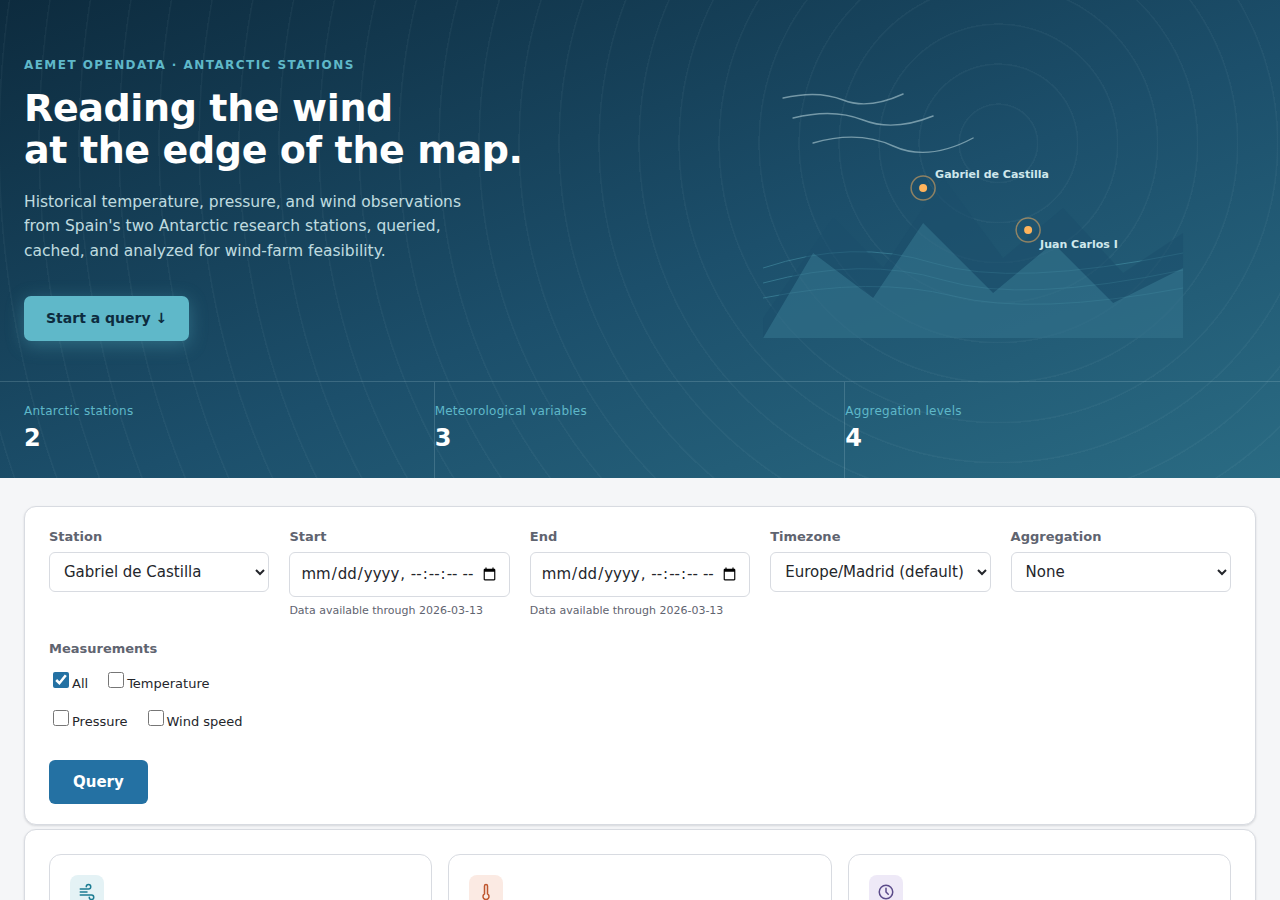
\includegraphics[width=0.92\textwidth]{../screenshots/empty-state.png}
\caption{The idle-state landing page: the full-bleed polar hero with the
station-marked coastline illustration, the query form, and the three
measurement explainer cards, before any query has been submitted. The
timezone field defaults to \texttt{Europe/Madrid}, and both date fields
already show a ``data available through'' caption sourced from
\texttt{GET /observations/latest-available} (Section~\ref{sec:latest-available}).}
\label{fig:empty-state}
\end{figure}

Figure~\ref{fig:empty-state} shows this idle state as actually rendered:
the query form sits directly below the hero, so the transition from
``understanding what this tool does'' to ``using it'' requires no
navigation, only scrolling, which the hero's own call-to-action button
performs programmatically.

Once a query is submitted, the hero is unmounted, not merely hidden, and
replaced by a compact header (\texttt{CompactHeader}) carrying the same
visual identity in a slim strip, present across the loading, success, and
error states alike. This distinction (unmount versus hide) matters for a
concrete reason discovered during development: an earlier version of this
transition left the page with no header at all once results were showing,
because the hero component was conditionally rendered only in the idle
branch and nothing replaced it, so the page briefly went headless between
submitting a query and results appearing. \texttt{CompactHeader} exists
specifically to close that gap, ensuring the page always carries its
identity regardless of request state.

Every measurement carries one consistent color identity across the entire
frontend, applied via shared CSS custom properties rather than
per-component literal color values: wind speed in cyan/teal, temperature
in warm orange-red, pressure in indigo/violet, used identically for chart
lines, KPI card accent rails, measurement-checkbox swatches, and chart
legends. Color is never the only signal carrying information; every
colored element also carries an explicit text label, since color alone is
not an accessible encoding for a value someone needs to act on.

\begin{figure}[htbp]
\centering
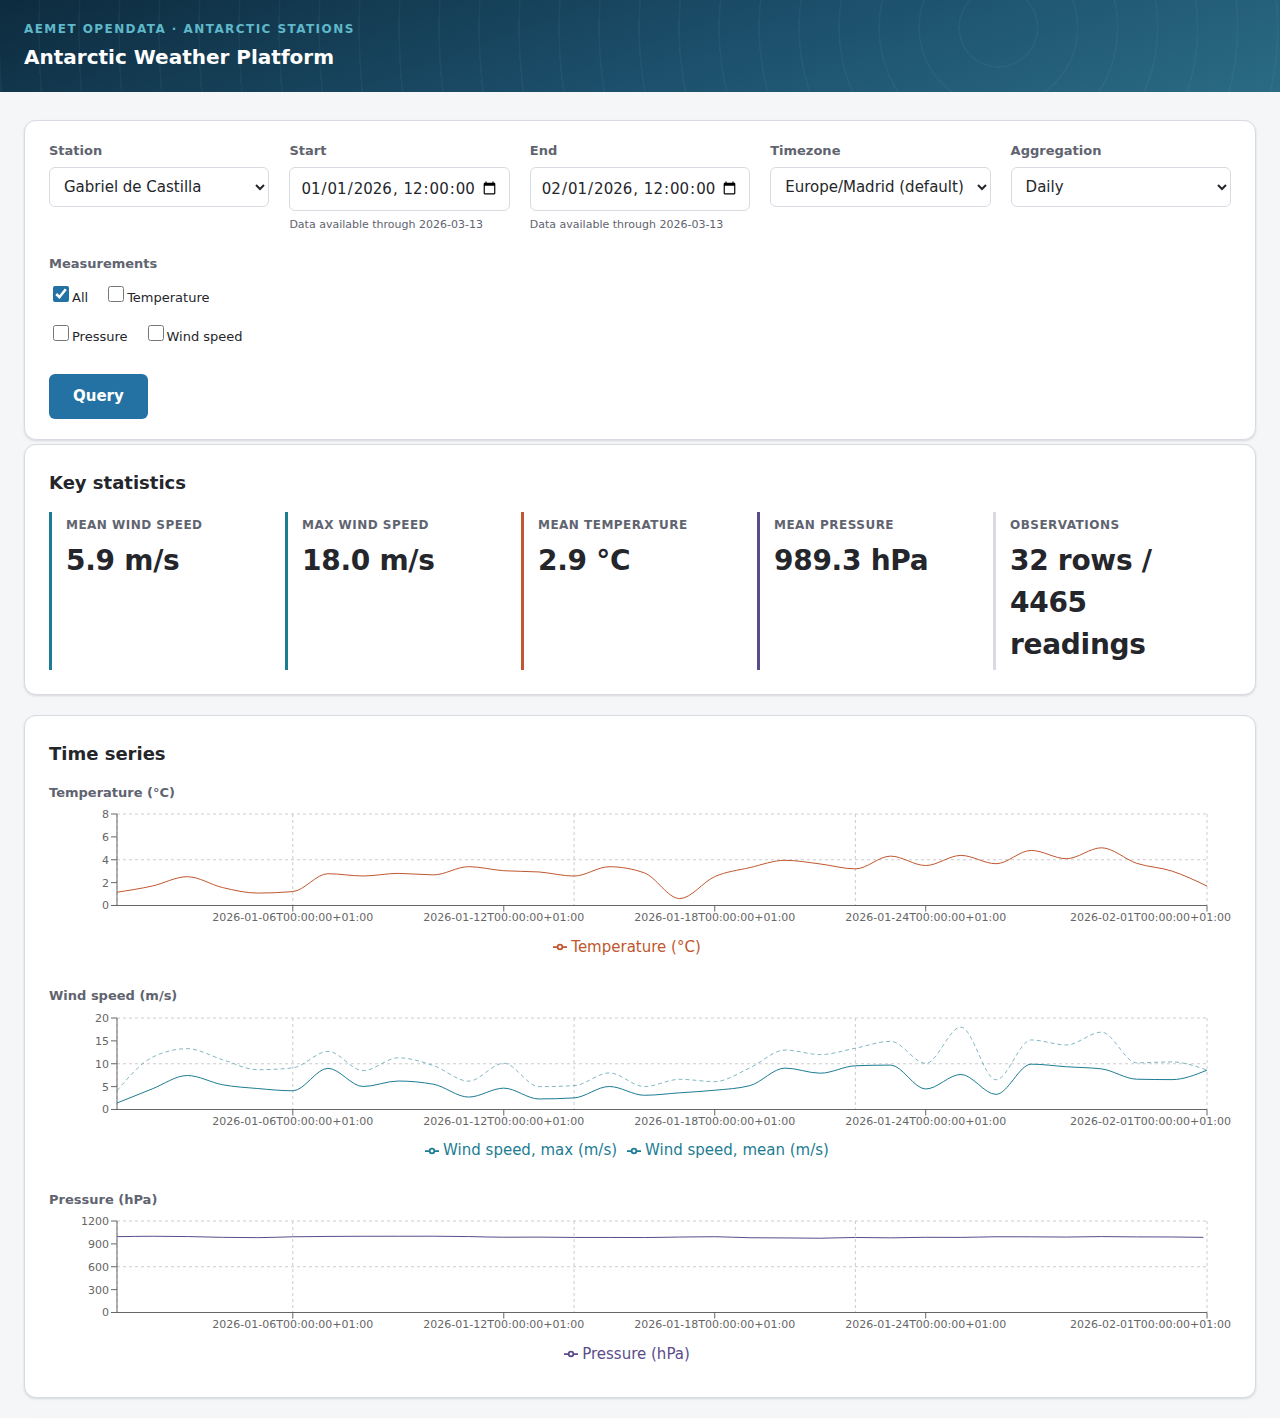
\includegraphics[width=0.92\textwidth]{../screenshots/results-kpi-wind.png}
\caption{A successful query for Gabriel de Castilla, daily aggregation,
January 2026: the compact header (replacing the hero, never leaving the
page headless), the query form retaining the submitted values, the KPI
strip with color-coded accent rails per measurement family, and the three
synchronized time-series panels (temperature, wind speed mean/max,
pressure). The dashed line in the wind panel is the bucket maximum,
sharing wind's own hue rather than a separate color, so ``mean vs.\ max''
reads as one measurement family, not two (Section~\ref{sec:aggregation}).}
\label{fig:results-kpi-wind}
\end{figure}

\begin{figure}[htbp]
\centering
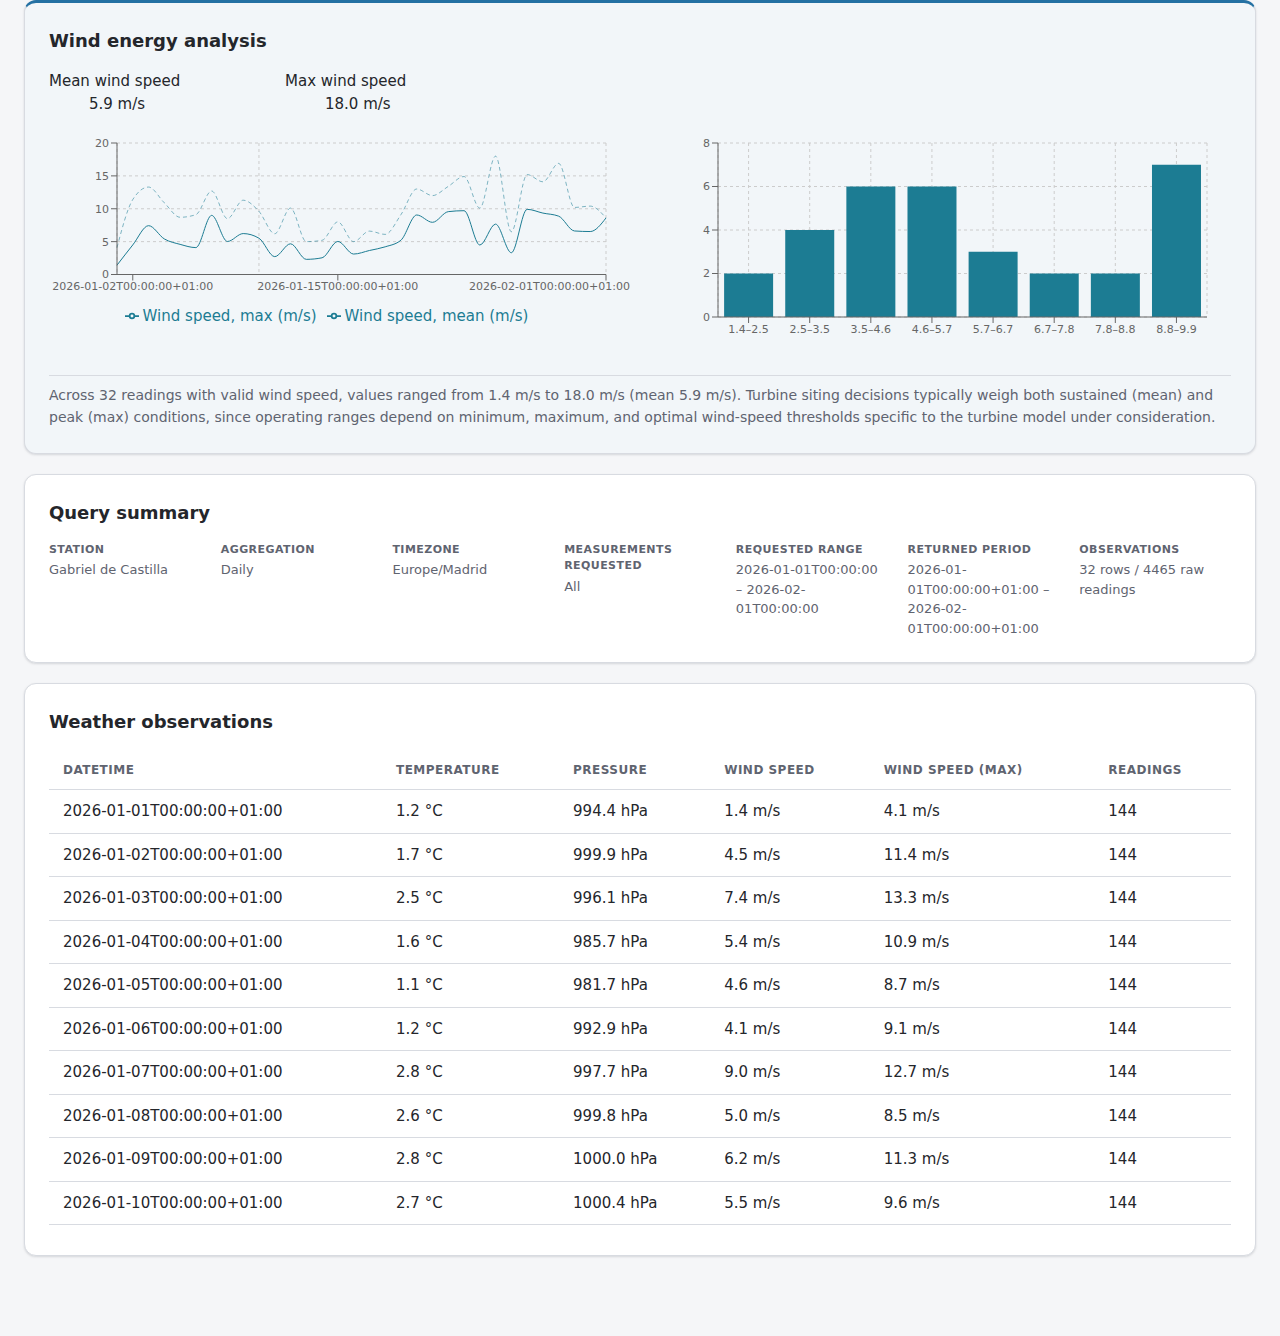
\includegraphics[width=0.92\textwidth]{../screenshots/results-timeseries-table.png}
\caption{The same query, scrolled further down: the wind-energy analysis
section (mean/max summary, a reused wind time series, and a client-side
histogram of the wind-speed distribution), the query-metadata summary
strip, and the observations table. No turbine-specific threshold (cut-in,
rated, or cut-out speed) is printed anywhere in this view, deliberately
(Section~\ref{sec:tradeoffs}).}
\label{fig:results-timeseries-table}
\end{figure}

Figures~\ref{fig:results-kpi-wind} and~\ref{fig:results-timeseries-table}
together show the full analytical workspace a successful query produces,
in the order \texttt{App.tsx} actually renders it: KPI strip, time series,
wind-energy analysis, query summary, then the table.

\section{Continuous Integration and Engineering Quality}
\label{sec:ci}

Two GitHub Actions workflows
(\texttt{.github/workflows/backend.yml}, \texttt{frontend.yml}) run on
every push and pull request touching their respective directory, each
scoped by a \texttt{paths} filter so a frontend-only change does not
trigger the backend job and vice versa. The backend workflow installs the
project (\texttt{pip install -e ".[dev]"}), then runs \texttt{ruff check},
\texttt{mypy} in strict mode, and \texttt{pytest} in that order, so a lint
failure is reported before a slower type-check or test run even starts.
The frontend workflow runs \texttt{npm ci} (a clean, lockfile-exact
install, deliberately not \texttt{npm install}, so CI never silently drifts
from what \texttt{package-lock.json} actually pins), then
\texttt{eslint}, \texttt{vitest run}, and finally \texttt{npm run build},
which itself invokes \texttt{tsc -b} as a build prerequisite, so a type
error fails the workflow at the build step without a separate, redundant
\texttt{tsc --noEmit} invocation.

These workflows were added late in development, after the AEMET
integration, timezone/DST handling, aggregation, caching, and frontend
work described in the preceding sections were already complete, not from
the project's first commit. This is stated plainly rather than left for a
reviewer to reconstruct from the commit history, consistent with this
report's policy throughout of describing what actually happened rather
than what would read best.

What existed for most of the implementation period, and what the 142
backend and 98 frontend tests, strict-mode type checking, and linting
referenced throughout this report were never contingent on, was the same
checks run manually and consistently by the developer: every backend
change was verified against \texttt{pytest}, \texttt{mypy} in strict mode,
and \texttt{ruff} before being considered complete, and every frontend
change against \texttt{vitest}, \texttt{tsc}, and \texttt{eslint} in the
same way. That discipline was real, and it is the reason the test and
type-check counts cited throughout this report are trustworthy even for
the sections written before CI existed, but it depended on the developer
remembering to apply it on every single change, with no independent
mechanism verifying that a given commit actually passed everything before
being pushed.

Automating that already-existing discipline into a pipeline that runs on
every push and pull request, rather than only when manually invoked, is
what closes the gap: a broken commit now shows as a failing check on
GitHub itself, rather than being discoverable only by a reviewer who
happens to clone the repository and run the suites by hand. The workflows
formalize a standard that was already being met, rather than introducing
one that was not.

\section{Security Considerations}
\label{sec:security}

The application's attack surface is small and mostly bounded by what it
does not do: it has no user authentication, no user-supplied data is
persisted beyond the AEMET observations themselves, and it serves exactly
one read-only endpoint plus a health check. The concrete measures actually
in place are:

\begin{itemize}[nosep]
    \item \textbf{Secrets never committed.} The AEMET API key is read
    exclusively from an environment variable
    (\texttt{app/core/config.py}); \texttt{.env} is covered by
    \texttt{.gitignore}, and only \texttt{.env.example} (containing no
    real key) is committed.
    \item \textbf{Startup-time configuration validation.} A missing or
    malformed required setting fails immediately when the application
    starts, with a clear error, rather than surfacing later as a confusing
    failure the first time a request happens to need that setting.
    \item \textbf{CORS is explicitly scoped}, not left at a permissive
    default: \texttt{CORS\_ALLOW\_ORIGINS} defaults to only
    \texttt{http://localhost:5173} (the local Vite dev server) and the
    middleware permits only \texttt{GET} requests, matching the fact that
    this API exposes no mutating operation at all.
    \item \textbf{No secret ever reaches a client or an error response.}
    5xx error responses return a generic message; the real exception
    detail, which could otherwise leak an internal table name, a config
    variable, or an upstream URL, is logged server-side only
    (Section on Error Handling, \texttt{README.md}).
    \item \textbf{Input validation at the boundary.} Every caller-supplied
    value (station, datetime format, timezone name, aggregation level,
    measurement selection) is validated before reaching any business
    logic, returning 400 with a descriptive message for a domain
    validation failure and 422 for a request FastAPI itself cannot parse,
    rather than allowing malformed input to propagate into the timezone or
    aggregation pipeline where a failure would be harder to trace back to
    its actual cause.
\end{itemize}

What this application deliberately does not need, given its actual
deployment shape (a local, single-user development tool, not a
multi-tenant public service): rate limiting on its own API (the AEMET
client's own outbound rate limiting, Section~\ref{sec:retry-strategy}, is
the relevant concern here, not inbound traffic to this application),
a reverse proxy in front of the development server, or any credential
storage, since it has no accounts to protect. These are not oversights;
they are scoped out because nothing in this system's actual deployment
target creates the risk they would mitigate.

\section{Scalability Considerations}
\label{sec:scalability}

The current design targets the challenge's actual stated scale: a
single-user or small-team tool querying two stations' historical data,
backed by SQLite. Several choices were made specifically because a more
scalable alternative was not justified at this scale, each with a stated
evolution path rather than being closed off by the current design:

\begin{itemize}[nosep]
    \item \textbf{SQLite, not PostgreSQL.} SQLite has no meaningful
    concurrent-write story, which is irrelevant here since this
    application has exactly one writer (the fetch-and-cache path) and
    reads are cheap. If concurrent write access ever became a real
    requirement, the repository's interface (\texttt{ObservationRepository})
    already isolates all persistence behind method calls with no SQL
    leaking into the service layer, so migrating the underlying engine to
    PostgreSQL would not require changing \texttt{WeatherService} or
    anything above it.
    \item \textbf{Cache-coverage checked with a single-range containment
    query, not an interval tree} (Section~\ref{sec:caching}). The
    complexity cost of a general interval-merging cache is not justified
    by the current single-query-at-a-time usage pattern; if usage patterns
    changed to include many overlapping, non-adjacent range requests
    per station, this is the first place a more general algorithm would
    be introduced.
    \item \textbf{Fetching on request, not a background ingestion
    worker.} Data is fetched from AEMET lazily, on the first request that
    needs an uncached range, rather than proactively ingested on a
    schedule. This keeps the system simple (no scheduler, no job queue) at
    the cost of the first request for any new range paying AEMET's
    latency directly. A background worker performing scheduled ingestion
    is a natural evolution if this system needed to guarantee low latency
    on every request, including the first one for a given range.
    \item \textbf{No caching layer in front of SQLite.} Query volume in
    this application's actual context does not approach a level where
    SQLite's own read performance is a bottleneck; introducing Redis or an
    equivalent hot-path cache ahead of that point would be optimizing a
    dimension that is not currently the constraint.
\end{itemize}

Grouping and reduction inside \texttt{aggregate} are both $O(n)$ in the
number of raw observations, which is the relevant complexity bound for a
bounded date-range query at $\sim$10-minute granularity, at most a few
thousand points even for a multi-year request once chunked, so this was
not a dimension requiring further optimization at this scale.

\section{Trade-offs and Limitations}
\label{sec:tradeoffs}

This section states the deliberate trade-offs already reasoned through
elsewhere in this report in one place, together with genuine limitations
not otherwise framed as decisions:

\begin{itemize}[nosep]
    \item \textbf{Single-range cache containment} over a general interval
    algorithm (Section~\ref{sec:caching}): correct and explainable for the
    actual usage pattern, but a request spanning two non-adjacent
    previously-fetched ranges is a full miss rather than a partial hit.
    \item \textbf{\texttt{httpx} over \texttt{httpx2}} for the production
    AEMET client, keeping \texttt{httpx2} only as a \texttt{TestClient}
    dev dependency (README, Trade-offs): a small amount of forward-risk
    accepted (building on a library with a long release gap) to avoid an
    unverified migration under real project time constraints.
    \item \textbf{No background ingestion, no distributed cache}
    (Section~\ref{sec:scalability}): appropriate to the current scale,
    with a stated evolution path if that scale changed.
    \item \textbf{Verification is scoped to two specific stations.} The
    AEMET response mapping treats every field outside the five actually
    used as optional, which was necessary because Gabriel de Castilla and
    Juan Carlos I were confirmed \emph{not} to return an identical field
    set (Section~\ref{sec:aemet-integration}), but this has only been
    verified against these two stations specifically, since they are the
    only two the specification requires.
    \item \textbf{The wind-farm feasibility framing informs presentation,
    not a modeling claim.} Reporting both mean and maximum wind speed,
    and building a dedicated wind-energy analysis view
    (Section~\ref{sec:frontend}), makes the data more useful for a
    feasibility assessment, but the system deliberately never states a
    specific turbine's cut-in, rated, or cut-out threshold, since those
    are turbine-model-specific figures outside this API's or the
    challenge's actual scope; a regression test in the frontend suite
    asserts that no such figure ever appears in the wind-energy view.
\end{itemize}

\section{Future Improvements}
\label{sec:future}

This section separates two different kinds of future work. Section~\ref{sec:future-hardening}
lists improvements that directly close a limitation already stated
elsewhere in this report, ordered by the same proportionality reasoning
applied throughout: the highest-value item first, each tied to a specific
section rather than asserted in isolation. Section~\ref{sec:future-extensions}
is more speculative and product-facing, describing how the system could
grow if the engagement extended beyond the challenge's current two-station,
single-user scope; these are explicitly framed as directions, not
commitments, and none of them is implied to be a small change.

\subsection{Hardening: closing the gaps already stated in this report}
\label{sec:future-hardening}

\begin{enumerate}[nosep]
    \item \textbf{A required-status-check branch rule on \texttt{main}},
    now that the CI workflows themselves exist (Section~\ref{sec:ci}):
    the workflows currently report status on every push and pull request,
    but nothing yet blocks a merge if either one fails, so completing this
    means configuring GitHub's branch protection to require both checks
    to pass before a pull request can merge, converting a reported signal
    into an enforced gate.
    \item \textbf{General interval-coverage caching}, if real usage ever
    showed the single-range containment scope limit
    (Section~\ref{sec:caching}) mattering in practice: a query pattern
    with genuinely overlapping, non-adjacent historical ranges per
    station would justify the added complexity of interval-tree
    reasoning that is not currently justified.
    \item \textbf{Scheduled background ingestion}, replacing the current
    fetch-on-request model (Section~\ref{sec:scalability}), if low
    first-request latency ever became a hard requirement rather than an
    accepted trade-off.
    \item \textbf{Broader station-field verification}, extending the
    empirical field-availability check performed for Gabriel de Castilla
    and Juan Carlos I (Section~\ref{sec:aemet-integration}) to any
    additional AEMET stations, should this system's scope ever extend
    beyond the two the challenge specifies.
    \item \textbf{A reverse proxy and inbound rate limiting}, appropriate
    if this system's deployment shape ever changed from a local,
    single-user tool toward a shared or public-facing service
    (Section~\ref{sec:security}).
\end{enumerate}

\subsection{Further ideas: growing beyond the challenge's current scope}
\label{sec:future-extensions}

\subsubsection{A dedicated mobile experience, not just a responsive layout}

The current frontend is usable on a narrow viewport (the layout stacks
rather than breaks), but it was designed and tested primarily against a
desktop-width browser, and the three-panel synchronized time series in
particular (Section~\ref{sec:frontend}) is not the right visualization for
a phone-width screen: three stacked charts each losing most of their
horizontal resolution is a worse reading experience than a single chart
with a measurement switcher. A genuine mobile treatment would mean
re-deriving the chart layout for small viewports rather than reflowing the
existing one, likely a single active-measurement chart with a
segmented control to switch between temperature, wind, and pressure, plus
touch-appropriate target sizes throughout the query form (the current
native \texttt{<input type="datetime-local">} controls already inherit
correct touch behavior from the browser, but the measurement checkboxes
and timezone dropdown were sized and spaced for a mouse cursor). This is a
real, separate design pass, not a CSS media-query afterthought, which is
exactly why it is scoped here as future work rather than attempted within
the current timeline.

\subsubsection{Database management: from a single SQLite file to an operable store}

Section~\ref{sec:scalability} already states why SQLite is the right
choice at the current scale (one writer, cheap reads, zero operational
overhead) and names PostgreSQL as the natural next engine if concurrent
write access ever became a real requirement. Beyond that specific
migration, a longer-lived deployment of this system would need database
\emph{management}, not just a bigger engine: a defined backup and
restore procedure for \texttt{weather.db} (currently a single file with no
automated backup at all, acceptable only because every row it contains is
independently re-derivable from AEMET on demand), a real migration tool
(Alembic, already named as the natural fit in the README's production
evolution path) once the schema has any change history worth tracking
instead of the current create-if-missing startup behavior, and basic
storage observability, table sizes, row counts per station, and cache
growth rate over time, so a future maintainer could answer ``is the cache
doing its job'' from a dashboard rather than by querying SQLite directly.
None of this is required at the challenge's current scale (two stations,
one deployment, one developer), which is precisely why it belongs here
rather than in the hardening list above.

\subsubsection{Timezone and location adaptability beyond the two Antarctic stations}

The timezone pipeline (Section~\ref{sec:timezone-dst}) was built to be
general on purpose, accepting either an IANA name or a fixed UTC offset,
resolving DST correctly, and always normalizing output to a single fixed
zone, even though the current system only ever needs to reason about
Europe/Madrid as that fixed output zone and two fixed-location Antarctic
stations as the data source. That generality was a deliberate choice
(Section~\ref{sec:timezone-dst}), and it is what makes a genuine next step
tractable rather than a rewrite: adding a third station, in any timezone,
would not touch \texttt{domain/time.py} at all, since the module already
treats ``which named zone is the fixed output'' as a parameter, not a
hardcoded assumption, even though \texttt{OUTPUT\_TIMEZONE} is currently
set as a module-level constant rather than a request-time or
per-deployment setting. Making that constant configurable, and pairing it
with a station registry (station identifier, display name, AEMET code,
and, critically, the station's own local timezone) instead of the current
two-member \texttt{Station} enum, would let this same domain logic serve
any AEMET station, or in principle any similarly-shaped meteorological
API, anywhere in the world, without touching the aggregation or DST
correctness logic that is this system's actual hard-won correctness
guarantee. This reframes the current two-station scope not as a
limitation of the architecture but as a deliberate, narrow instantiation
of a pipeline that was already built general enough to outgrow it.

\section{Conclusion}

This system was built by treating AEMET's actual, live behavior, not its
documentation or the challenge specification's own field table, as the
final source of truth for every implementation decision that touched the
external API: the two-step response indirection, the \texttt{"NaN"}
sentinel, the undocumented quality flag, the undocumented $\sim$31-day
range limit, and the multi-retry 429 behavior were each discovered or
confirmed empirically before being encoded into the client, and each is
covered by a test that pins down the specific behavior discovered rather
than a generic assumption about how an API like this ``should'' work.

The same verification-first discipline was applied internally: the two
DST hazards are handled by round-tripping through UTC and checking for
disagreement, not by trusting Python's defaults; the two SQLite
correctness bugs (timezone loss on round-trip, an upsert targeting the
wrong key) were both caught by tests specifically designed to catch a
class of subtle, silent bug, not merely to exercise the happy path; and
every deliberate scope limitation, from single-range cache containment to
the choice not to model wind direction, is stated as a reasoned trade-off
with its own evolution path, rather than left implicit or discovered only
by a reviewer reading the code.

For a period during development, this report stated a genuine gap rather
than a considered trade-off: the absence of a CI pipeline
(Section~\ref{sec:ci}), acknowledged plainly rather than described as
done, consistent with this report's own premise that a technical report
exists to be checked against running code, not to present the most
flattering account available. That gap is now closed; the remaining item,
gating merges on the workflows' own status rather than only reporting it,
is recorded honestly as future work (Section~\ref{sec:future-hardening})
rather than folded into a claim of completeness it does not yet earn.

\end{document}
